% ==========================================
% AutoExtraction Source: 02-18-wednesday.mp4
% Model: gemini-3-flash-preview
%
% MERGED AND CLEANED by Gemini Code Assist on 2026-05-01
% This file combines TEIL 1, TEIL 2, and TEIL 3 to create a coherent transcript,
% removing redundant overlapping sections and applying final polish.
% ==========================================


\lecturechapter{Wednesday}{Feb 18th}{February 18th 2026}{Metric Spaces: Sequences and Completeness}

\begin{nice-box}[Context]
This lecture continues the exploration of Metric Spaces, transitioning from the foundational axioms of distance to the rigorous study of sequences, convergence, and accumulation points. The lecturer emphasizes the continuity of concepts from Analysis 1, now generalized to arbitrary sets equipped with a metric.
\end{nice-box}

% ==========================================
% SECTION 1: SEQUENCES IN METRIC SPACES
% ==========================================
\section{Sequences in Metric Spaces}

\begin{spoken-clean}[00:00:00 - 00:00:50]
So, uh, hopefully by the second week it will all take us two seconds to go from chatting, uh, to full silence. So, uh, we will continue with metric spaces, provided my voice allows. Uh, remember last time we introduced this pair \inlinemetanote{points at the board}: $(X, d)$. $X$ is a set and $d$ was a map from $X \times X$ to positive numbers, or non-negative numbers. And now for today, you can forget about the rest of math you learned, because we are going to use only this and the three axioms. So, you just need to remember three pieces of information: the three axioms.
\end{spoken-clean}

\begin{math-stroke}[Foundational Metric Space]
We operate within a metric space defined by the pair:
\[ (X, d) \]
where $X$ is a set and $d: X \times X \to [0, \infty)$ is a distance function satisfying the three fundamental axioms (identity of indiscernibles, symmetry, and the triangle inequality).
\end{math-stroke}

\subsection{Definition of a Sequence}

\begin{spoken-clean}[00:00:50 - 00:01:50]
So, uh, now we will learn again concepts you, uh, you saw in Analysis 1, and the first concept is that of sequence. \inlinemetanote{Writes on the board} Definition: sequence. You saw sequences of real numbers, uh, so if $X$ is a set, we define — we call sequence in $X$ a map that we put like this: $x$ from the natural numbers to $X$. This is small $x$, this is big $X$, okay?
\end{spoken-clean}

\begin{math-stroke}[Definition: Sequence]
\begin{definition}[Sequence]\label{def:sequence}
Let $X$ be a set. A \emph{sequence} in $X$ is a mapping from the set of natural numbers $\mathbb{N}$ to the set $X$:
\[ x: \mathbb{N} \to X \]
\end{definition}
\end{math-stroke}

\begin{spoken-clean}[00:01:50 - 00:03:00]
And as in Analysis 1, instead of denoting this map $x(n)$ as we do with functions, we will use these notations: $x_n$, right? Sub-index. And when we will — when we want to denote the full map, the — this is just one element, the $n$, the $n$-th element of the sequence. This is the $n$-th element that belongs to $X$, belongs to the set $X$, capital $X$. And when we want to denote the full sequence, we will say: let $(x_n)$ like this be a sequence, and then we can put this, we can put this \inlinemetanote{writes various notations on the board}. So, all of these are equivalent notations. Or we can put, I don't know, things like that. So, this is our notation for sequence, right?
\end{spoken-clean}

\begin{math-stroke}[Sequence Notation]
While a sequence is formally a function, we typically employ subscript notation to denote its elements.
\begin{description}
    \item[Individual Element:] $x_n$ represents the $n$-th element of the sequence, where $x_n \in X$.
    \item[Full Sequence:] To denote the entire sequence, the following notations are considered equivalent:
    \begin{itemize}
        \item $(x_n)_{n \ge 0}$
        \item $(x_n)_{n=0}^{\infty}$
        \item $(x_n)_{n \in \mathbb{N}}$
    \end{itemize}
\end{description}
\end{math-stroke}

\subsection{Convergence and Limits}

\begin{spoken-clean}[00:03:00 - 00:04:11]
But now we are in a — in a metric space, so we can define also convergent sequence and limit. Definition number two will be: convergent sequence and limit. \inlinemetanote{Writes on the board} So, we say $(x_n)$ — so this is for a metric space, so $(X, d)$ is a metric space, $d$ is the distance, and $(x_n)_{n \ge 0}$ has limit $x$ in $X$ if... well, we can put it in many ways.
\end{spoken-clean}

\begin{math-stroke}[Definition: Convergence and Limit]
\begin{definition}[Convergence and Limit]\label{def:convergence-limit}
Let $(X, d)$ be a metric space. A sequence $(x_n)_{n \ge 0}$ in $X$ is said to \emph{converge} to a limit $x \in X$ if the distance between the sequence elements and the limit point approaches zero:
\[ d(x_n, x) \to 0 \quad \text{as real numbers}. \]
\end{definition}
\end{math-stroke}

\begin{spoken-clean}[00:04:11 - 00:05:15]
But essentially what we will say is that if we — if we have a sequence of points in our space, it converges to our given limit point if the distance converges to zero. We have the distance, we need to phrase everything in terms of the distance. So, if the distance between $x_n$ and the limit point converges to zero as real numbers, right? These are — these are points in your abstract space, but the distance between the two points is a number. So, I can say if this distance goes to zero, uh, this means that this point is the limit of that sequence.
\end{spoken-clean}

\begin{didactic-insight}[The Bridge to Real Numbers]
The lecturer highlights a crucial conceptual bridge: while $x_n$ and $x$ are elements of an abstract set $X$, the distance $d(x_n, x)$ is always a real number. This allows us to use the familiar notion of limits from $\mathbb{R}$ to define convergence in any metric space.
\end{didactic-insight}

\begin{spoken-clean}[00:05:15 - 00:06:23]
So, equivalently, if you want something very similar, equivalently: for all $\epsilon$ positive, exists capital $N$ that depends on $\epsilon$, such that the distance between $x_n$ and $x$ is less than $\epsilon$ whenever $n$ is bigger than capital $N$, right? This is the same, more analogous to what you have seen in Analysis 1 for sequences. Okay. But now this is super general because we saw last time that metric spaces could be a space of functions, could be anything. Now you know how to do sequence — convergent sequences in any, uh, in very general setup.
\end{spoken-clean}

\begin{math-stroke}[Formal \texorpdfstring{$\epsilon$}{epsilon}-N Definition of Convergence]
The convergence $x_n \to x$ is formally defined as:
\[ \forall \epsilon > 0, \exists N(\epsilon) \in \mathbb{N} \text{ s.t. } \forall n \ge N, d(x_n, x) < \epsilon \]

\begin{explanation-of-steps}
This definition mirrors the classical definition of convergence in $\mathbb{R}$, replacing the absolute difference $|x_n - x|$ with the general metric $d(x_n, x)$. It states that for any arbitrarily small distance $\epsilon$, there exists a point in the sequence beyond which all subsequent elements are \qt{trapped} within an $\epsilon$-neighborhood of the limit $x$.
\end{explanation-of-steps}
\end{math-stroke}

% \begin{ai-global-state-checkpoint-invisible-content}
% timestamp: 00:06:00
% topic: Definitions of sequences and convergence in metric spaces.
% board_state: def:sequence, def:convergence-limit
% next_goal: Establish uniqueness of limits.
% open_loops: none
% \end{ai-global-state-checkpoint-invisible-content}

\begin{spoken-clean}[00:06:23 - 00:07:38]
Okay, so, uh, now we know — well, let me once and for all give you the notations we will use. So, when the — when the ambient, when the — when the space you are using is clear, most of the time in this course will be $\mathbb{R}^n$ with the Euclidean distance, or maybe the complex numbers that is $\mathbb{R}^2$, right? Um, then we will write to say that, uh, $x_n$ has limit $x$, we will use these notations: that limit in $n$, or when $n$ goes to infinity, of $x_n$ is equal to $x$. This we can write when — when everything is clear from the context, right? When the $X$ and the distance. Or we can also put even shortly: $x_n$ converges to $x$. This I like a lot because it is very compact. Right? As in here, I used it in here. Okay.
\end{spoken-clean}

\begin{math-stroke}[Limit Notation]
When the metric space $(X, d)$ is understood, we use the following standard notations for the limit:
\begin{itemize}
    \item $\lim_{n \to \infty} x_n = x$
    \item $x_n \to x$
\end{itemize}
\end{math-stroke}

% ==========================================
% SECTION 2: UNIQUENESS OF LIMITS
% ==========================================
\section{Uniqueness of Limits}

\begin{spoken-clean}[00:07:38 - 00:09:12]
Now, we define — given a convergent sequence, we define — or we said what is its limit. Now, first question: is the limit unique? Let's start for the very, very basic, uh, fundamental questions. So, first lemma. \inlinemetanote{Writes on the board} Oh, nice. What is this? Um, is — so, Lemma: the limit of a sequence is unique. Let's say: if — so in a metric space $(X, d)$, right? And now you take a sequence $(x_n)_{n \ge 0}$, and you have that $x_n$ converges to $x$ and you know also that $x_n$ converges to $y$, two points, given points of $X$. $x, y$ in $X$. So, this is a sequence, and this is an assumption. Assume that $x_n$ converges to $x$ and $x_n$ converges to $y$. Then $x = y$. Right?
\end{spoken-clean}

\begin{nice-box}[Lemma: Uniqueness of the Limit]
\begin{lemma}[Uniqueness of the Limit]\label{lem:uniqueness-limit}
In any metric space $(X, d)$, if a sequence $(x_n)$ converges to $x$ and also converges to $y$, then $x$ must be equal to $y$.
\end{lemma}
\end{nice-box}

\begin{spoken-clean}[00:09:12 - 00:11:03]
So, how do we prove this? \inlinemetanote{Draws a sketch on the board} So, these are two potential limit points, $x$ and $y$. And remember that the first axiom of the distance says that the distance distinguishes the points. So, the distance between two points is positive. So, let me call the distance between $x$ and $y$, I will call it $2 \times \epsilon$ (i.e., $d(x, y) = 2\epsilon$) that is a positive number. All right? Or to make — to make it more dramatic, I can put $3 \times \epsilon$. And also more symmetric, because the $3$ and the $\epsilon$ are symmetric. Okay. Um, then this is $3\epsilon$. Now, the definition of convergence tells us that after a certain point — so for very, very large $n$ — all the elements of the sequence will fall close to the limit. But at the same time, all the elements of the sequence will fall close to that limit. And this should contradict another axiom that is the triangle inequality. Okay? Here we see the intuition. So, all the elements cannot be at the same time here and here, right? So, this is what we are going to do. And now we write — we write this in symbols using the definition, right?
\end{spoken-clean}

\begin{math-stroke}[Intuition for Uniqueness Proof]
\begin{center}
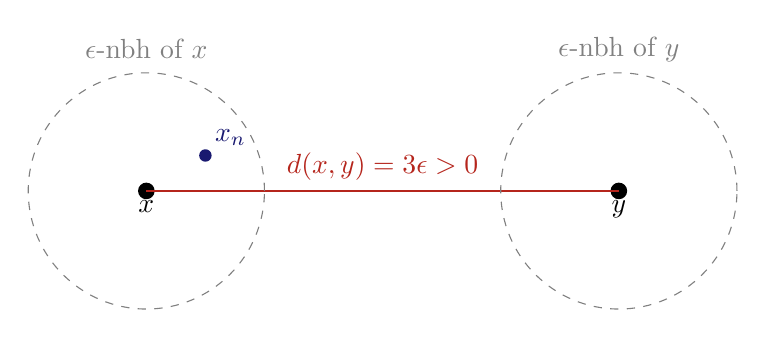
\begin{tikzpicture}[scale=1.5]
% \begin{ai-tikz-planner-invisible-content}
% 1. Background: Points x and y.
% 2. Midground: A point x_n representing a sequence element.
% 3. Foreground: Dashed circles of radius epsilon around x and y.
% 4. Annotations: Labels for x, y, x_n and the total distance 3*epsilon.
% \end{ai-tikz-planner-invisible-content}
    % Points x and y
    \coordinate (X) at (0,0);
    \coordinate (Y) at (4,0);
    \fill (X) circle (2pt) node[below] {$x$};
    \fill (Y) circle (2pt) node[below] {$y$};

    % Distance line
    \draw[thick, BrickRed] (X) -- (Y) node[midway, above] {$d(x, y) = 3\epsilon > 0$};

    % Neighborhoods
    \draw[dashed, gray] (X) circle (1cm);
    \draw[dashed, gray] (Y) circle (1cm);
    \node[gray] at (0, 1.2) {$\epsilon$-nbh of $x$};
    \node[gray] at (4, 1.2) {$\epsilon$-nbh of $y$};

    % Sequence point x_n
    \coordinate (Xn) at (0.5, 0.3);
    \fill[MidnightBlue] (Xn) circle (1.5pt) node[above right] {$x_n$};
\end{tikzpicture}
\end{center}

\begin{explanation-of-steps}
The proof relies on a contradiction. If $x \neq y$, their distance $d(x, y)$ is some positive value, say $3\epsilon$. For sufficiently large $n$, $x_n$ must be within $\epsilon$ of $x$ AND within $\epsilon$ of $y$. However, the triangle inequality dictates that the total distance $d(x, y)$ cannot exceed the sum of the distances $d(x, x_n) + d(x_n, y)$, which would imply $3\epsilon < 2\epsilon$—a clear contradiction.
\end{explanation-of-steps}
\end{math-stroke}

\begin{spoken-clean}[00:11:03 - 00:12:38]
So, by definition of the limit, exists — so given that $\epsilon$ over there, exists $N$ — let's say $N_x$ — such that the distance between $x_n$ and $x$ is less than $\epsilon$ for all $n$ bigger than $N_x$, right? And the same with $y$: exists some $N_y$ such that the distance between $x_n$ and $y$ is less than $\epsilon$ for all $n$ bigger than or equal to $N_y$. And then if I take capital $N$ to be the maximum of these two numbers, what happens? That for all $n$ bigger than or equal to $N$, it is bigger than both, so I will have the distance between $x$ and $y$ — this was what? This by definition was $3 \times \epsilon$. Right? Now I can use the triangle inequality with these three points: $x, y$ and $x_n$. So, this is less than or equal to the distance between $x$ and $x_n$ plus the distance between $x_n$ and $y$. I'm using the triangle axiom. Now I want to have this, right? So, I need to switch these two arguments. So, I'm using the second axiom here: the symmetry. So, axiom number three, triangle inequality; axiom number two, I can switch the points in the distance. And then I get that this is less than $\epsilon + \epsilon$. So, $3\epsilon$ is less than $2\epsilon$, contradiction. So, the contradiction comes from the fact that I assumed that the points are different and the distance is positive. If the points are the same and the distance is zero, there is no contradiction, of course. So, this finishes the proof of the uniqueness of the limit.
\end{spoken-clean}

\begin{proof}[Formal Proof: Uniqueness of Limits]
\begin{math-stroke}
Assume $x_n \to x$ and $x_n \to y$ with $x \neq y$. By the first metric axiom, $d(x, y) > 0$. Let $d(x, y) = 3\epsilon$ for some $\epsilon > 0$.
By the definition of convergence:
\begin{itemize}
    \item $\exists N_x \in \mathbb{N}$ such that $\forall n \ge N_x, d(x_n, x) < \epsilon$.
    \item $\exists N_y \in \mathbb{N}$ such that $\forall n \ge N_y, d(x_n, y) < \epsilon$.
\end{itemize}
Let $N = \max(N_x, N_y)$. Then for all $n \ge N$, both conditions hold. Applying the triangle inequality (Axiom 3) and symmetry (Axiom 2):
\begin{align*}
3\epsilon = d(x, y) &\le d(x, x_n) + d(x_n, y) \\
&= \underbrace{d(x_n, x)}_{< \epsilon} + \underbrace{d(x_n, y)}_{< \epsilon} \\
&< \epsilon + \epsilon = 2\epsilon
\end{align*}
This yields $3\epsilon < 2\epsilon$, which is a contradiction since $\epsilon > 0$. Thus, our assumption $x \neq y$ must be false, and $x = y$.
\end{math-stroke}
\end{proof}

% \begin{ai-global-state-checkpoint-invisible-content}
% timestamp: 00:12:00
% topic: Proof of uniqueness of limits.
% board_state: lem:uniqueness-limit, eq:triangle-inequality-proof
% next_goal: Address student confusion on the contradiction.
% open_loops: student question about the last line of the proof.
% \end{ai-global-state-checkpoint-invisible-content}

\begin{spoken-clean}[00:12:38 - 00:14:14]
Um, can you — can you tell me now — how is the — how is this pace? Is it very slow? Is it very quick? Is it okay? Yeah, good. So, it's important I tell you because I have the experience from two years ago: there are some people that whatever I do, they always find it super slow, right? And these are the people that sometimes are more active looking at me and giving feedback. So, it's very important that if people start to be confused, before it's too late, I know. And in this direction, today there will be the election of the — before the break, I think it's today — there will be the election of the class speakers. And this is very useful, and I ask you to volunteer because then I have a more fluid communication. Maybe some people don't come to complain to me that I'm going too fast or too slow, but then you can go to your speakers and they will give feedback. And like this we will adjust as we go.
\end{spoken-clean}

\begin{student-interaction}
I do not quite understand where the contradiction is. So, why this proof actually works. I do not get the last line you wrote there.
\end{student-interaction}

\begin{spoken-clean}[continued]
This last line? \inlinemetanote{points at the board} Yes. Okay. This is the definition of $3\epsilon$. Now, the triangle inequality says that when you have three points, the distance between two of them is shorter than going from one to the third and to the third to the second. Right? This is the triangle. This is less than or equal to. Now, if we switch these two and we use that and that, the switching is by the second axiom, I can switch the two points. And I get less than $\epsilon + \epsilon$. So, I am getting that $3\epsilon$ is less than $2\epsilon$, which is a contradiction, right? Okay. So, the only place where I could — where the contradiction came from is because I assumed that the points are different and the $\epsilon$ is positive. If the $\epsilon$ is zero, you cannot do that. Okay?
\end{spoken-clean}

% ==========================================
% SECTION 3: SUBSEQUENCES AND ACCUMULATION POINTS
% ==========================================
\section{Subsequences and Accumulation Points}

\subsection{Definition of a Subsequence}

\begin{spoken-clean}[00:15:32 - 00:17:23]
So, next thing that — that you learned in Analysis 1 is definition: subsequence. It will be the same. Right? If $(x_n)$ is a sequence in a set $X$, we define — so is there some problem or some...? You have some, yeah? No? No, but it's important — is there some confusion with this proof? I can spend more time, we have time. Yeah, good. \inlinemetanote{The lecturer retrieves the catch-box microphone} So, now is the tricky part, right? Almost. \inlinemetanote{Tosses microphone to student}
\end{spoken-clean}

\begin{student-interaction}
Um, so can we use the terminology of limit if $x$ isn't in the set $X$? So, for example, if we have like $\mathbb{R}$ but without zero and like $x_n$ is defined as $1/n$, it converges to zero but zero isn't in $X$.
\end{student-interaction}

\begin{spoken-clean}[continued]
No, in this context, no. Okay. So, here you — you can use because your ambient — so you are artificially removing part of your set, but you can measure the distance between zero and the positive numbers because you are in $\mathbb{R}$, and $\mathbb{R}$ has its distance. But by the definition, you see, when you look at the definition, all the things that appear in the definition need to have a meaning. And when you have the distance of $x_n$ and $x$ goes to zero, so that this number is a real number is well-defined, you need the both points to be in your space. Otherwise, I don't know what is the distance between something that lives in one space and something that lives in another galaxy, right? Okay.
\end{spoken-clean}

\begin{math-stroke}[Definition: Subsequence]
\begin{definition}[Subsequence]\label{def:subsequence}
Let $(x_n)_{n \ge 0}$ be a sequence in a set $X$. A \emph{subsequence} is any sequence of the form:
\[ (x_{f(n)})_{n \ge 0} \]
where $f: \mathbb{N} \to \mathbb{N}$ is a strictly increasing function.
\end{definition}

\begin{explanation-of-steps}
A strictly increasing map $f$ ensures that we are picking elements from the original sequence in their original relative order, but potentially skipping some. Formally, $f$ satisfies:
\[ f(n) < f(m) \iff n < m \]
In standard notation, we often write $n_k$ instead of $f(k)$, denoting the subsequence as $(x_{n_k})_{k \ge 0}$.
\end{explanation-of-steps}
\end{math-stroke}

% \begin{ai-global-state-checkpoint-invisible-content}
% timestamp: 00:18:00
% topic: Subsequences and Accumulation Points.
% board_state: def:subsequence, def:accumulation-point
% next_goal: Explain the relationship between accumulation points and subsequences.
% open_loops: student question about epsilon-delta vs sequence definitions.
% \end{ai-global-state-checkpoint-invisible-content}

\subsection{Accumulation Points}

\begin{spoken-clean}[00:17:23 - 00:18:44]
So, something you already learned in $\mathbb{R}$ also: accumulation points. You know what is an accumulation point. Let's put in here. Definition: accumulation points. And we will give two things, two definitions. So, if $Y$ is a subset of $X$ — I will not write every time, but now unless — so every time $(X, d)$ is a metric space. And $Y$ is a subset of $X$, subset. We say that $y$ in $X$ is an accumulation point of $Y$ if exists a sequence $(y_n)$ contained in $Y$ such that $y_n$ converges to $y$. Bullet point number one. And bullet point number two is for sequence. So, if $(x_n)$ is a sequence of $X$, we say the $x$ is an accumulation point of this sequence if exists a subsequence that converges to $x$.
\end{spoken-clean}

\begin{math-stroke}[Definition: Accumulation Points]
\begin{definition}[Accumulation Point]\label{def:accumulation-point}
Let $(X, d)$ be a metric space.
\begin{description}
    \item[For a Set:] A point $y \in X$ is an \emph{accumulation point} of a subset $Y \subseteq X$ if there exists a sequence $(y_n)_{n \ge 0}$ with $y_n \in Y$ for all $n$, such that:
    \[ \lim_{n \to \infty} y_n = y \]
    \item[For a Sequence:] A point $x \in X$ is an \emph{accumulation point} of a sequence $(x_n)_{n \ge 0}$ if there exists a subsequence $(x_{n_k})_{k \ge 0}$ such that:
    \[ \lim_{k \to \infty} x_{n_k} = x \]
\end{description}
\end{definition}
\end{math-stroke}

\begin{spoken-clean}[00:00:36 - 00:01:43]
So, uh, you will notice that I'm going — I'm going very slowly, uh, speaking slowly, writing slowly, but I'm writing — I'm not writing very much on the blackboard. The reason — I'm giving you a lot of time to see if what I write makes sense, but I'm not writing a lot because when I start later to increase the speed and write like this \inlinemetanote{gestures quickly}, you will need to follow, right? So, uh, if — if something is not clear because I need to write more — I say everything speaking, right? But I don't write everything on the blackboard. If someone is confused, raise your hand, stop me, we have time. Okay? But this will be very useful, for instance, I use abbreviations or things like that. So, later when I want to go a slightly quicker, this will be very useful that — that we are all used to that. Yeah.
\end{spoken-clean}

\begin{meta-note}[Classroom Interaction]
The lecturer retrieves the catch-box microphone to prepare for a student question.
\end{meta-note}

\begin{student-interaction}
Um, is there a reason why we often use for definitions something we kind of learned in Analysis 1 as corollaries or lemmas? For example, for the accumulation point, we usually saw the definition with this $\epsilon$-$\delta$ thing and that whenever you have this $\delta$-neighborhood around your point and find the intersection with $Y$, the set is not empty. Is there a reason why we avoid $\epsilon$-$\delta$?
\end{student-interaction}

\begin{spoken-clean}[00:02:12 - 00:03:12]
No, there is no reason. With the limit, no. Um, the $\epsilon$-$\delta$ was more usually for continuity, right? In the continuity we will see the sequence, the $\epsilon$-$\delta$, we will see that everything is equivalent. Here you cannot do that much $\epsilon$-$\delta$. You can use $\epsilon$s or you can use limits, and in the notion of limit the $\epsilon$ is implicit. Because when I gave the definition of limit there was an $\epsilon$ — I gave with the $\epsilon$ and without the $\epsilon$. But no, it should be exactly equivalent as in Analysis 1. When there is something like that that you have more than one possibility, as when we define the continuity of maps, of functions, I will give all the equivalent definitions systematically. But here, there are no $\epsilon$-$\delta$s that I can see yet.
\end{spoken-clean}

\begin{meta-note}[Transition]
The lecturer erases the left and center chalkboards to begin a new derivation.
\end{meta-note}

% ==========================================
% SECTION 4: CHARACTERIZING CONVERGENCE VIA ACCUMULATION POINTS
% ==========================================
\section{Characterizing Convergence via Accumulation Points}

\begin{spoken-clean}[00:03:13 - 00:05:03]
Uh, let me prove something. Easy lemma. So, a sequence — this is to emphasize also that a sequence in general is not convergent. So, it will have several accumulation points. Many. So, when a sequence is convergent, it is exactly when the sequence has only one accumulation point. And this is something you know for — for real numbers, and now we see it is the same in a metric space.
\end{spoken-clean}

\begin{math-stroke}[Lemma: Convergence and Accumulation Points (Initial State)]
\begin{nice-box}[Board Action]
The lecturer writes the first version of the lemma on the board.
\end{nice-box}
\begin{lemma}\label{lem:convergence-acc-point-v1}
\textcolor{red}{\text{(Incorrect Statement)}} \\
A sequence $(x_n)_{n \ge 0} \subset X$ in a metric space $(X, d)$ converges to $x$ if and only if $x$ is its sole accumulation point.
\[ x_n \to x \iff x \text{ is its only acc. pt.} \]
\end{lemma}
\end{math-stroke}

\begin{spoken-clean}[00:05:04 - 00:06:50]
So, let's prove that. Proof. \inlinemetanote{Writes on the board} So, what we need to show is that, um, $x_n$ converges to $x$ is equivalent — I will put it in this phrasing — $x_n$ converges to $x$ is equivalent to: for every accumulation point — it is a limit of a subsequence, right? For every convergent subsequence $(x_{n_k})$ converging to $y$ for some $y$, is $y = x$? Right? I'm rephrasing this and I'm rephrasing this. I'm saying these two things are equivalent. Now, there should be one implication that is easy, right? Because I can take $x_{n_k}$ could be $x_n$, right? I could take the — the full sequence is always a partial subsequence of the — it's the case that $f$ is the identity, $f(n) = n$. Taking this, I find that $x_n$ converges to $x$. So, this proves this implication \inlinemetanote{points at the board}. Just taking a particular case of a subsequence.
\end{spoken-clean}

% \begin{ai-global-state-checkpoint-invisible-content}
% timestamp: 00:06:00
% topic: Lemma relating convergence to accumulation points.
% board_state: lem:convergence-acc-point-v1
% next_goal: Prove the equivalence.
% open_loops: student question about the validity of the lemma.
% \end{ai-global-state-checkpoint-invisible-content}

\begin{proof}[Proof of Lemma \ref{lem:convergence-acc-point-v1} (Partial)]
\begin{math-stroke}
We aim to show the equivalence:
\[ x_n \to x \iff \left( \forall (x_{n_k}) \text{ s.t. } x_{n_k} \to y \implies y = x \right) \]
The implication $(\impliedby)$ is considered trivial by the lecturer:
If every convergent subsequence must converge to $x$, then since the sequence $(x_n)$ is a subsequence of itself (where $f = \id$), it must also converge to $x$.
\end{math-stroke}
\end{proof}

\begin{student-interaction}
In the first implication we show to the left... how do we know $x_n$ is convergent? Because we assume that any convergent subsequence converges to $x$, but we do not know that $x_n$ is convergent a priori.
\end{student-interaction}

\begin{spoken-clean}[00:08:16 - 00:09:30]
So, you say... ah, okay. So, every convergent subsequence converges to $x$. Uh, maybe I phrased the lemma... I wanted to... so, now you are asking me a — so, let me think again. A sequence $x_n$ converges to $x$... yes, I said that $x$ is the only accumulation point. Yeah. And you are telling me... so, if I take a subsequence that converges to $y$, I know that $y$ is $x$. Good. But you are telling me why the full sequence should be a convergent subsequence? Good. Good question. Well spotted. Um, yes, I had in mind a slightly weaker result and then I stated... this is also true, but then this implication is a bit harder. Okay. Very good, very good. We can discuss.
\end{spoken-clean}

\begin{didactic-insight}[The "False" Lemma]
The lecturer intentionally (or accidentally) states a lemma that is subtly incorrect in general metric spaces without further assumptions like compactness. This creates a \qt{circus} moment where a student spots a logical gap, forcing a more rigorous re-evaluation of the relationship between accumulation points and convergence.
\end{didactic-insight}

\begin{spoken-clean}[00:09:31 - 00:11:23]
Okay, so this is a — yeah. Can you throw there? Yeah, let's — let's have all the questions and then we will try to solve all of them. Okay. It's a very good discussion. Yeah. \inlinemetanote{Tosses microphone to another student}
\end{spoken-clean}

\begin{student-interaction}
So, what would happen if you take a sequence that for even $n$ is just $n$, and for odd $n$ is $1/n$? Because then you have an accumulation point at zero, but the entire sequence has no limit. What happens then?
\end{student-interaction}

\begin{spoken-clean}[continued]
\inlinemetanote{The lecturer pauses to think, looking at the board} Okay. Let me — let me ask this question out loud, okay? Because... so, you say, okay, we have $\mathbb{R}$ \inlinemetanote{writes on the board}. And you take this sequence that for $n$ equal — so for, let's say, $x_{2n} = n$ and then $x_{2n+1} = 1/n$, right? This is the question. And then you say this sequence satisfies that every accumulation point — you say is only zero, right? Because this is unbounded, this goes to infinity. And then every subsequence, it seems to satisfy this. Yeah. Good question.
\end{spoken-clean}

\begin{math-stroke}[Counter-example to Lemma \ref{lem:convergence-acc-point-v1}]
The student provides a counter-example in $\mathbb{R}$ to show that having a unique accumulation point does not imply convergence:
Consider the sequence $(x_n)_{n \ge 0}$ defined by:
\[
x_n = \begin{cases} 
n & \text{if } n \text{ is even} \\
\frac{1}{n} & \text{if } n \text{ is odd}
\end{cases}
\]
\begin{explanation-of-steps}
For this sequence, the only accumulation point is $0$ (from the odd terms). The even terms $x_{2n} = 2n$ diverge to infinity and thus do not contribute any accumulation points in $\mathbb{R}$. However, the full sequence $(x_n)$ clearly does not converge to $0$ because the even terms grow without bound. Thus, the condition \qt{sole accumulation point} is insufficient for convergence in non-compact spaces.
\end{explanation-of-steps}
\end{math-stroke}

\begin{spoken-clean}[00:11:24 - 00:13:40]
Good, let's put all — any other question? We will try to solve all of them. Okay. It's a very good discussion. Yeah. I mean, in the — in the script, something is slightly different. We assume that every subsequence converges to $x$. We don't say that $x$ is the only accumulation point. Which would be correct, but this is... yeah, this is the — the stronger statement I was talking about. So, what script are you looking at? At the one from two years ago? Because it says that we assume that every subsequence converges to $x$. Yeah, this is much easier. And actually is true. Okay. So, every subsequence converges to $x$.
\end{spoken-clean}

\begin{nice-box}[Board Action]
The lecturer writes \qt{FALSE} over the first lemma and writes two new, corrected versions.
\end{nice-box}
\begin{color-box}{black}
\textbf{FALSE}
\end{color-box}
\begin{math-stroke}[Correcting the Lemma]
\begin{lemma}[Lemma 1 - Corrected]\label{lem:convergence-acc-point-v2}
A sequence $(x_n)_{n \ge 0} \subset X$ converges to $x$ if and only if every subsequence $(x_{n_k})_{k \ge 0}$ converges to $x$.
\[ x_n \to x \iff \forall (x_{n_k})_{k \ge 0}, x_{n_k} \to x \]
\end{lemma}

\begin{explanation-of-steps}
This version is trivially true because the sequence itself is a subsequence. If every subsequence converges to $x$, then the sequence must converge to $x$. Conversely, if the sequence converges to $x$, any selection of its elements (a subsequence) must also converge to $x$.
\end{explanation-of-steps}
\end{math-stroke}

% \begin{ai-global-state-checkpoint-invisible-content}
% timestamp: 00:12:00
% topic: Correcting the lemma on convergence and accumulation points.
% board_state: lem:convergence-acc-point-v2, lem:bw-related
% next_goal: Introduce Lemma 3 (Bolzano-Weierstrass related).
% open_loops: none
% \end{ai-global-state-checkpoint-invisible-content}

\begin{spoken-clean}[00:13:41 - 00:15:50]
But what I wanted to put — Lemma 3, that is a bit more interesting, is that if $x_n$... so, the same assumptions. Same assumptions as above. Then $x_n$ converges to $x$ if and only if every subsequence $(x_{n_k})$ has a sub-subsequence — so a subsequence of the subsequence — such that $x_{n_{k_l}}$ converges to $x$. So, whenever I take a — I can choose a subsequence, maybe this subsequence does not converge. But then, we will see next day the definition of compact spaces — and you know in $\mathbb{R}$. So, in compact spaces, like here in your example, you have realized that your example, you could do this example because the space is unbounded. The $\mathbb{R}$ is unbounded. Or is not compact, right? If you restrict to a compact interval of $\mathbb{R}$, what I wrote here was true. So, we see it's not completely false, it just we need some extra assumptions. In a compact space that is complete — but you will learn this today — in a complete space that is compact, this will be true. But we need some extra assumptions. Instead, this thing — is true always. Every subsequence $(x_{n_k})$ has a sub-subsequence that converges to $x$, then the limit is $x$. Right? And since today I need to do other things, and this is a good — it's a bit difficult but it's a good exercise, we will do that. I will put this statement as exercise. You try to solve it, and then the next day or in a couple of days when many people have tried, I will solve it for you here. And we will discuss again. But like this you can practice a bit. It's a good exercise. It's not trivial, that one. This one is a bit easy, is the one I gave. Is easier.
\end{spoken-clean}

\begin{math-stroke}[Lemma 3: Sub-subsequence Characterization]
\begin{lemma}[Sub-subsequence Characterization of Convergence]\label{lem:sub-subsequence}
Under the same assumptions as above, a sequence $(x_n)_{n \ge 0}$ converges to $x$ if and only if every subsequence $(x_{n_k})_{k \ge 0}$ contains a further subsequence (a \qt{sub-subsequence}) $(x_{n_{k_l}})_{l \ge 0}$ that converges to $x$:
\[ x_n \to x \iff \forall (x_{n_k})_{k \ge 0}, \exists (x_{n_{k_l}})_{l \ge 0} \text{ s.t. } x_{n_{k_l}} \to x \]
\end{lemma}
\end{math-stroke}

\begin{nice-box}[Exercise]
The lecturer marks Lemma \ref{lem:sub-subsequence} as an \qt{exercise} for the students to solve before the next lecture.
\end{nice-box}

\begin{meta-note}[Transition]
The lecturer erases the right chalkboard to transition to the next major topic: Completeness.
\end{meta-note}

% ==========================================
% SECTION 5: COMPLETE METRIC SPACES
% ==========================================
\section{Complete Metric Spaces}

\begin{spoken-clean}[00:15:51 - 00:17:20]
Actually, this false lemma is very appropriate because it will allow me to — so it will be a very good example to introduce two concepts. The next concept I'm going to introduce is the concept of complete space. Right? Complete space. We know that $\mathbb{R}^n$ is complete — we know that $\mathbb{R}$ is complete, sorry. Um, this we proved in Analysis 1. And now you are going to see the definition of complete space like in this abstract level, and we will prove that $\mathbb{R}^n$ is complete. Okay.
\end{spoken-clean}

\subsection{Cauchy Sequences}

\begin{spoken-clean}[00:17:21 - 00:18:48]
So, first we need to define Cauchy sequence. Cauchy sequence. \inlinemetanote{Writes on the board} So, it's the same definition as in $\mathbb{R}$, right? So, $(x_n)_{n \ge 0}$ is Cauchy — a sequence is Cauchy if for all $\epsilon$ positive, exists capital $N$ such that the distance between $x_n$ and $x_m$ is less than $\epsilon$ whenever $n$ and $m$ are both bigger than $N$. Right? If you wait enough --- so if both indices are sufficiently large, then the two --- the two points, any two points of the sequence become close. Right? This is the same as in $\mathbb{R}$. And now when you know Cauchy sequence, we can define a complete --- so complete space. \inlinemetanote{Writes on the board} We say that $(X, d)$ is complete if every sequence --- every Cauchy sequence converges to some limit in the space. Right?
\end{spoken-clean}

\begin{math-stroke}[Definition: Complete Metric Space]
\begin{definition}[Cauchy Sequence]\label{def:cauchy-sequence-v2}
A sequence $(x_n)_{n \ge 0}$ in a metric space $(X, d)$ is \emph{Cauchy} if:
\[ \forall \epsilon > 0, \exists N \in \mathbb{N} \text{ s.t. } d(x_n, x_m) < \epsilon \quad \text{whenever } n, m \ge N \]
\end{definition}

\begin{definition}[Complete Metric Space]\label{def:complete-space-v2}
A metric space $(X, d)$ is \emph{complete} if every Cauchy sequence in $X$ converges to a limit $x \in X$.
\end{definition}
\end{math-stroke}

\begin{spoken-clean}[00:01:25 - 00:02:26]
This fact that it converges to some limit in the space I can put in the parenthesis, because in my definition of convergence we say that the sequence converges if there is a point of the space towards which it is converging. So, whenever I say that a sequence converges, it's to some point in the space. We cannot remove points from the space. So, if we start to remove points, as your peer was asking before, what happens if I take the positive numbers? Okay, then I'm taking a complete space that is $\mathbb{R}$ and I'm making it incomplete by removing points, right?
\end{spoken-clean}

\begin{spoken-clean}[00:02:26 - 00:03:12]
So, here we get that if the Cauchy sequence doesn't converge, then the metric space is not complete. Exactly. But my question is: what does it mean for a Cauchy sequence to not converge? I can give you some example. Let's give some examples of non-complete spaces that you know very well. Okay?
\end{spoken-clean}

\begin{student-interaction}
So, here we get that if the Cauchy sequence doesn't converge, then the metric space is not complete?
\end{student-interaction}

\begin{spoken-clean}[continued]
Exactly.
\end{spoken-clean}

\begin{meta-note}[Transition]
The lecturer erases the left and center chalkboards to prepare for examples of completeness.
\end{meta-note}

% ==========================================
% SECTION 6: EXAMPLES OF (IN)COMPLETE SPACES
% ==========================================
\section{Examples of (In)complete Spaces}

\begin{spoken-clean}[00:04:05 - 00:05:24]
So, example of complete space we have $\mathbb{R}$, right? We have $\mathbb{R}$ with the distance --- the Euclidean distance. \inlinemetanote{Writes on the board} What is the Euclidean distance in $\mathbb{R}$? Is the distance between two numbers is just the absolute value of the difference, right? And now we take a subset of $\mathbb{R}$. $A$ subset $\mathbb{R}$. Then we can restrict the distance to $A$, the absolute value of the difference. Now, so let's say that Case number one: $A$ equals, say, $(0, \infty)$. Is this complete?
\end{spoken-clean}

\begin{math-stroke}[Example: The Open Interval \texorpdfstring{$(0, \infty)$}{(0, inf)}]
Consider the set $A = (0, \infty) \subset \mathbb{R}$ equipped with the standard Euclidean metric:
\[ d(x, y) = |x - y| \]
\begin{center}
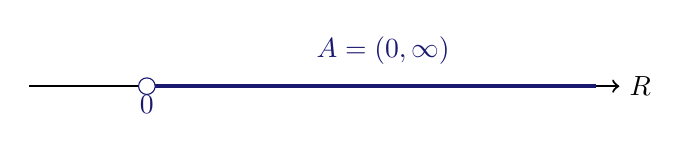
\begin{tikzpicture}[scale=1.5]
% \begin{ai-tikz-planner-invisible-content}
% 1. Background: Horizontal axis.
% 2. Midground: Open interval (0, inf) drawn with a thick line and an open parenthesis at 0.
% 3. Foreground: Point 0 marked as excluded.
% \end{ai-tikz-planner-invisible-content}
    \draw[->, thick] (-1,0) -- (4,0) node[right] {$\mathbb{R}$};
    \draw[ultra thick, MidnightBlue] (0,0) -- (3.8,0);
    \node[MidnightBlue, below] at (0,0) {$0$};
    \draw[MidnightBlue, fill=white] (0,0) circle (2pt); % Open boundary
    \node[MidnightBlue] at (2, 0.3) {$A = (0, \infty)$};
\end{tikzpicture}
\end{center}
\end{math-stroke}

\begin{spoken-clean}[00:05:24 - 00:06:15]
What is the problem here? This is not complete because you are missing the zero. So, you --- so this is open, right? And you can have a Cauchy sequence, the sequence $x_n = 1/n$. \inlinemetanote{Writes on the board} This sequence is Cauchy, and the limit would be zero, but you are removing the limit from your space. So, this space is not complete. Right?
\end{spoken-clean}

\begin{math-stroke}[Incompleteness of \texorpdfstring{$(0, \infty)$}{(0, inf)}]
The space $(A, d)$ is \emph{not complete}.
\begin{description}
    \item[Cauchy Sequence:] Consider $x_n = \frac{1}{n}$ for $n \ge 1$.
    \item[Limit in $\mathbb{R}$:] In the ambient space $\mathbb{R}$, $\lim_{n \to \infty} x_n = 0$.
    \item[Failure of Completeness:] Since $0 \notin A$, the sequence does not converge to any point within the metric space $(A, d)$.
\end{description}
\end{math-stroke}

% \begin{ai-global-state-checkpoint-invisible-content}
% timestamp: 00:06:00
% topic: Examples of incomplete spaces (open intervals).
% board_state: def:cauchy-sequence-v2, def:complete-space-v2, ex:open-interval-incomplete
% next_goal: Discuss closed intervals and the rational numbers.
% open_loops: none
% \end{ai-global-state-checkpoint-invisible-content}

\begin{spoken-clean}[00:06:15 - 00:07:34]
Instead, if you take a closed set, let's say $[a, b]$ closed, a closed interval, then as a metric space with the distance of the absolute value, this is a complete metric space. Because when you take a Cauchy sequence, a Cauchy sequence converges in $\mathbb{R}$, so the limit will belong to $\mathbb{R}$, but then since this is a closed interval, the limit will belong to your space. Right? More interesting example: $\mathbb{Q} \subset \mathbb{R}$. So, $A = \mathbb{Q}$. If the subset is $\mathbb{Q}$, the rational numbers, the rational numbers are not complete. That's because you can take a sequence of rational numbers converging to $\sqrt{2}$, right?
\end{spoken-clean}

\begin{math-stroke}[Examples: Closed Intervals and Rational Numbers]
\begin{description}
    \item[Closed Intervals:] The space $A = [a, b]$ with the Euclidean metric is \emph{complete}. Any Cauchy sequence in $[a, b]$ converges to a limit in $\mathbb{R}$, and since the set is closed, that limit must lie within $[a, b]$.
    \item[Rational Numbers:] The space $(\mathbb{Q}, d)$ is \emph{not complete}.
    \begin{itemize}
        \item There exist sequences $(x_n) \subset \mathbb{Q}$ such that $x_n \to \sqrt{2}$ in $\mathbb{R}$.
        \item Such a sequence is Cauchy in $\mathbb{Q}$ (because it converges in the larger space $\mathbb{R}$), but its limit $\sqrt{2}$ is not in $\mathbb{Q}$.
    \end{itemize}
\end{description}

\begin{explanation-of-steps}
The incompleteness of $\mathbb{Q}$ was the primary historical motivation for the construction of the real numbers $\mathbb{R}$. We \qt{fill the holes} in $\mathbb{Q}$ to ensure that every sequence that \qt{should} converge actually has a limit point.
\end{explanation-of-steps}
\end{math-stroke}

\begin{spoken-clean}[00:07:34 - 00:09:25]
You can take some sequence of rational numbers that as real numbers converge to $\sqrt{2}$. So, if you were --- if your space were the rational numbers, the --- so the fraction, right? Just fractions of integers. And you didn't invent yet the --- the reals, you would have a problem because you try --- so you don't have this completeness property. And this is the whole point of inventing the reals, right? To make the rationals complete.
\end{spoken-clean}

\begin{meta-note}[Transition]
The lecturer erases the right chalkboard and prepares to state the main theorem of the section.
\end{meta-note}

% ==========================================
% SECTION 7: COMPLETENESS OF R^n
% ==========================================
\section{Completeness of \texorpdfstring{$\mathbb{R}^n$}{Rn}}

\begin{spoken-clean}[00:09:25 - 00:11:08]
Okay, so now I can do two things. So, I don't see more questions, right? So, we can --- we can start to introduce open and closed sets in a metric space. Okay? And then --- the last five minutes I will --- I will discuss a bit because this year you already saw with Professor Figalli the construction of the reals, uh, with these Dedekind cuts, I think, right? So, you have a construction of the real numbers, but one can also construct really as --- as I said here, as a completion. So, if you make $\mathbb{Q}$ complete, there is a --- a way, an abstract way to make any metric space complete. We can discuss this very quickly for those interested. And this procedure applies to $\mathbb{Q}$ and gives you $\mathbb{R}$. And this is another way to construct a model of $\mathbb{R}$. But since this is not strictly needed now, it's just for extra information, and I will rush and be quick on that, and I will spend just the last five minutes. Now let's advance and introduce open and closed sets. Ah, okay, or maybe I can --- no, I think that --- sorry, maybe now I can prove, it's better that I prove that $\mathbb{R}^n$ is complete. It's a good time.
\end{spoken-clean}

\begin{nice-box}[Theorem: Completeness of \texorpdfstring{$\mathbb{R}^n$}{Rn}]
\begin{theorem}\label{thm:rn-complete}
The space $\mathbb{R}^n$ equipped with the Euclidean distance $d_{\text{Eucl}}$ is a complete metric space.
\end{theorem}
\end{nice-box}

\begin{spoken-clean}[00:11:08 - 00:12:38]
So, let's say this theorem. \inlinemetanote{Writes on the board} Sorry. $\mathbb{R}^n$ with the Euclidean distance is complete. So, this is a theorem you have for $\mathbb{R}$. And actually, to prove the theorem for $\mathbb{R}^n$, I will use the result in $\mathbb{R}$. I will use that $\mathbb{R}$ is complete, that this is a highly non-trivial thing. It's almost axiomatic. You define --- you define at the beginning $\mathbb{R}$ axiomatically to make it complete. So, this is hard. But once I know that $\mathbb{R}$ is complete, it's very easy to show that $\mathbb{R}^n$ is complete. Right? So, I will prove this theorem, but to prove this theorem I will need some lemma that will be useful for you many, many times, that says the following.
\end{spoken-clean}

% \begin{ai-global-state-checkpoint-invisible-content}
% timestamp: 00:12:00
% topic: Completeness of R^n and the coordinate-wise convergence lemma.
% board_state: thm:rn-complete, lem:coordinate-convergence
% next_goal: State and prove the lemma relating vector convergence to coordinate convergence.
% open_loops: none
% \end{ai-global-state-checkpoint-invisible-content}

\subsection{Coordinate-wise Convergence}

\begin{spoken-clean}[00:12:38 - 00:14:12]
So, if $x_n$... ah, now we will have the usual notational problem. So, I will put $x_m$ \inlinemetanote{Writes on the board} a sequence in $\mathbb{R}^n$. I did not use sub-index $n$ here, because when I'm in $\mathbb{R}^n$, $n$ will be in this case the dimension. So, I cannot use $n$ here, okay? And then, when we have a sequence of points like this, $x_m$, remember that for a point in $\mathbb{R}^n$ --- so this is a bit of notation, but it's important that we clarify right now. So, in $\mathbb{R}^n$, we were denoting the points $x = (x_1, \dots, x_n)$. And these are the coordinates of the point that are $n$ real numbers.
\end{spoken-clean}

\begin{math-stroke}[Notation for Sequences in \texorpdfstring{$\mathbb{R}^n$}{Rn}]
To avoid conflict with the dimension $n$, we denote a sequence in $\mathbb{R}^n$ using the index $m$:
\[ (x_m)_{m \ge 0} \subset \mathbb{R}^n \]
Each element $x_m$ of the sequence is a vector with $n$ coordinates:
\[ x_m = (x_{m,1}, x_{m,2}, \dots, x_{m,n}) \]
where $x_{m,i} \in \mathbb{R}$ represents the $i$-th coordinate of the $m$-th vector in the sequence.
\end{math-stroke}

\begin{spoken-clean}[00:14:12 - 00:15:50]
But now, if I have a sequence of points, we will denote the coordinates like this: $x_m$ is a point in the sequence, and we will denote the coordinates $x_{m,1}, x_{m,2}, \dots, x_{m,n}$. \inlinemetanote{Writes on the board} You see, there is one sub-index that is which element of the sequence, and the second sub-index which coordinate. Right? It must be like that. So, this is the notation. And if you want, there is a small notational conflict because when you see $x_m$, you are not sure --- unless you --- well, you will be sure by the context. But if I only tell you $x_m$, what is this? Is the $m$-th coordinate of the point $x$, or the $m$-th element of a sequence? You will know always looking at the context. But this is a small notational conflict that I have pointed out in the notes also.
\end{spoken-clean}

\begin{nice-box}[Lemma: Coordinate-wise Convergence]
\begin{lemma}\label{lem:coordinate-convergence}
Let $(x_m)_{m \ge 0}$ be a sequence in $\mathbb{R}^n$. Then $x_m$ converges to $x$ if and only if every coordinate converges to the corresponding coordinate of the limit:
\[ x_m \to x \iff x_{m,i} \to x_i \quad \text{for all } i = 1, \dots, n \]
\end{lemma}
\end{nice-box}

\begin{spoken-clean}[00:15:51 - 00:17:20]
So, the way to find if a sequence converges in $\mathbb{R}^n$, it's just look at each coordinate, and if each coordinate is converging to the corresponding coordinate of the limit --- these are the coordinates of that, right? --- then you have the convergence, and this is if and only if. And we will first prove the lemma, and from this lemma we will get immediately that the $\mathbb{R}^n$ is complete. Okay.
\end{spoken-clean}

\begin{proof}[Proof of Lemma \ref{lem:coordinate-convergence}]
\begin{spoken-clean}[00:17:21 - 00:18:42]
Okay, let's do this implication, right? The implication to the right ($\implies$). So, I start --- starting point is I know that $x_m$ converges to $x$. What does it mean? \inlinemetanote{Writes on the board} For all $\epsilon$ positive, exists capital $N$ such that the modulus of $x_m - x$ is less than $\epsilon$ if $m$ is bigger than $N$. This is the definition of convergence in a metric space, and I'm using that in my metric space the distance is the modulus of the difference of points. So, this is the same as the distance between $x_m$ and $x$. It's the definition of the Euclidean distance. Right?
\end{spoken-clean}

\begin{math-stroke}[Proof: Implication \texorpdfstring{$\implies$}{=>}]
Assume $x_m \to x$. By definition:
\[ \forall \epsilon > 0, \exists N \in \mathbb{N} \text{ s.t. } \forall m \ge N, \|x_m - x\| < \epsilon \]
where $\| \cdot \|$ denotes the standard Euclidean norm.
\end{math-stroke}

% \begin{ai-global-state-checkpoint-invisible-content}
% timestamp: 00:18:00
% topic: Proof of the coordinate-wise convergence lemma.
% board_state: lem:coordinate-convergence, eq:norm-inequality
% next_goal: Show that coordinate difference is bounded by the vector norm.
% open_loops: none
% \end{ai-global-state-checkpoint-invisible-content}

\begin{spoken-clean}[00:18:42 - 00:20:12]
Now I want to prove that this implies that each coordinate converges. But you see that --- \inlinemetanote{Writes on the board} this thing implies that $|x_{m,i} - x_i|$ in absolute value... what is this? This is less than the sum for $j=1$ to $n$ of the root... no, the root goes outside. Of $(x_{m,j} - x_j)^2$. Right? If I take --- so given some $i$, so given $i$ in the set $\{1, \dots, n\}$, so given some coordinate $i$, $|x_{m,i} - x_i|$ is less than the sum for all coordinates of the squares and then you take the square root. Right? But this is the norm by definition. And I'm saying that this eventually --- so this will be less than $\epsilon$. Right?
\end{spoken-clean}

\begin{math-stroke}[Coordinate Bound by Norm]
For any fixed coordinate $i \in \{1, \dots, n\}$, we have the fundamental inequality:
\begin{equation}\label{eq:coord-norm-bound}
|x_{m,i} - x_i| = \sqrt{(x_{m,i} - x_i)^2} \le \sqrt{\sum_{j=1}^n (x_{m,j} - x_j)^2} = \|x_m - x\|
\end{equation}
\begin{explanation-of-steps}
The absolute difference of a single coordinate is always less than or equal to the total Euclidean distance between the vectors. Since $\|x_m - x\| < \epsilon$ for $m \ge N$, it follows immediately that $|x_{m,i} - x_i| < \epsilon$ for the same $m \ge N$. This proves that $x_{m,i} \to x_i$ for each $i$.
\end{explanation-of-steps}
\end{math-stroke}

\begin{spoken-clean}[00:20:12 - 00:21:30]
And this is what I wanted to show, right? Given $\epsilon$, exists some $N$ --- here is the same capital $N$ --- such that when $m$ is bigger than $N$, the coordinate --- the element $x_{m,i} - x_i$ will be less than $\epsilon$. This just follows by this inequality, the comparison between the difference of coordinates and the square root. So, this implication is rather easy and is done here. \inlinemetanote{Draws a Q.E.D. box for the first part}
\end{spoken-clean}

\begin{spoken-clean}[00:21:30 - 00:22:55]
And the other implication ($\impliedby$) is almost the same but is slightly harder. Because now I start at the other point. I know suppose that for each coordinate $i$, $x_{m,i}$ converges to $x_i$. So, I'm putting the definition. \inlinemetanote{Writes on the board} This means that for all $i$, given $i$, for all $\epsilon$ exists some $N$ that depends on $i$, that's why I call it $N_i$, such that this holds. Good. And now, if I can do it this, I can do it --- I can take $\epsilon$ divided by $n$, so I can take $\epsilon/n$, right? It's just you are taking a different $\epsilon$. This is true.
\end{spoken-clean}

\begin{math-stroke}[Proof: Implication \texorpdfstring{$\impliedby$}{<=}]
Assume $x_{m,i} \to x_i$ for all $i \in \{1, \dots, n\}$.
By definition, for each $i$:
\[ \forall \epsilon' > 0, \exists N_i \in \mathbb{N} \text{ s.t. } \forall m \ge N_i, |x_{m,i} - x_i| < \epsilon' \]
To prove vector convergence, we choose $\epsilon' = \frac{\epsilon}{\sqrt{n}}$.
\end{math-stroke}

\begin{spoken-clean}[00:22:55 - 00:24:45]
And then what you do now is that, okay, if this happens, then the modulus of $x_m - x$... what is this? This is the sum for $i=1$ to capital $n$ of $(x_{m,i} - x_i)^2$ square root. Now I'm saying that for if $m$ I will take $m$ bigger than the maximum for $i$ between $1$ and $n$ of these numbers $N_i$. I take the maximum of all these numbers, I call this $N$. If I take this $N$ that is the maximum of all these numbers and $m$ is larger, it would satisfy all the time at the same time all these conditions. And then I will get this is less than the root of $n$ times, and then this is $\epsilon^2$ over $n^2$. Each is less than $\epsilon/n$, so when I square is $\epsilon^2/n^2$. And this is less than $\epsilon$ divided by root $n$, that is less than $\epsilon$.
\end{spoken-clean}

\begin{math-stroke}[Vector Convergence from Coordinate Convergence]
Let $N = \max(N_1, N_2, \dots, N_n)$. Then for all $m \ge N$, the condition $|x_{m,i} - x_i| < \frac{\epsilon}{\sqrt{n}}$ holds for all $i$ simultaneously.
Substituting this into the Euclidean norm:
\begin{align*}
\|x_m - x\| &= \sqrt{\sum_{i=1}^n (x_{m,i} - x_i)^2} \\
&< \sqrt{\sum_{i=1}^n \left( \frac{\epsilon}{\sqrt{n}} \right)^2} \\
&= \sqrt{\sum_{i=1}^n \frac{\epsilon^2}{n}} \\
&= \sqrt{n \cdot \frac{\epsilon^2}{n}} = \sqrt{\epsilon^2} = \epsilon
\end{align*}
\begin{explanation-of-steps}
By choosing a sufficiently large $N$ such that every coordinate is \qt{close enough} to its limit, we ensure that the total Euclidean distance (the sum of the squared differences) is also small. This establishes that $x_m \to x$ in $\mathbb{R}^n$.
\end{explanation-of-steps}
\end{math-stroke}

\begin{spoken-clean}[00:24:45 - 00:25:20]
You see, this establishes that implication. So, I assumed that the coordinates converge, I needed to take a smaller $\epsilon$ divided by $n$, but then the vector converges. Right?
\end{spoken-clean}
\end{proof}

\begin{spoken-clean}[00:25:20 - 00:26:35]
And now, with exactly the same trick, exactly the same setup, I can prove the theorem. Proof of the theorem, today's theorem that is the completeness of $\mathbb{R}^n$. $\mathbb{R}^n$ complete. Right? So, how do you prove that something is complete? You need to take --- you give me a Cauchy sequence and I must show that the Cauchy sequence converges.
\end{spoken-clean}

\begin{proof}[Proof of Theorem \ref{thm:rn-complete}: Completeness of \texorpdfstring{$\mathbb{R}^n$}{Rn}]
\begin{math-stroke}
Let $(x_m)_{m \ge 0}$ be a Cauchy sequence in $\mathbb{R}^n$.
\begin{description}
    \item[Step 1: Coordinate-wise Cauchy:] By the inequality in Equation \ref{eq:coord-norm-bound}, for each $i \in \{1, \dots, n\}$:
    \[ |x_{m,i} - x_{k,i}| \le \|x_m - x_k\| \]
    Since $(x_m)$ is Cauchy in $\mathbb{R}^n$, it follows that each coordinate sequence $(x_{m,i})_{m \ge 0}$ is Cauchy in $\mathbb{R}$.
    \item[Step 2: Completeness of $\mathbb{R}$:] Since $\mathbb{R}$ is complete, each coordinate sequence converges to some $x_i \in \mathbb{R}$:
    \[ \lim_{m \to \infty} x_{m,i} = x_i \]
    \item[Step 3: Vector Convergence:] Define the vector $x = (x_1, \dots, x_n) \in \mathbb{R}^n$. By Lemma \ref{lem:coordinate-convergence}, since each coordinate converges, the vector sequence converges:
    \[ \lim_{m \to \infty} x_m = x \]
\end{description}
Thus, every Cauchy sequence in $\mathbb{R}^n$ converges, proving that $\mathbb{R}^n$ is complete.
\end{math-stroke}
\end{proof}

\begin{spoken-clean}[00:26:35 - 00:28:08]
So, in one sentence because it's time, the proof of the completeness of $\mathbb{R}^n$ is just pass to the components, look at the components, the components are Cauchy sequences, they converge, and then you put together the components to make the point and prove the existence of the limit. Right? I'm using the lemma, this implication.
\end{spoken-clean}

\begin{student-interaction}
Could you please elaborate why you use the minimum with the distances there instead of, for instance, the maximum?
\end{student-interaction}

\begin{spoken-clean}[00:28:12 - 00:28:47]
\inlinemetanote{The lecturer looks at the board} Uh... it's the maximum. Okay. Thank you. \inlinemetanote{Corrects the board} Thank you. \inlinemetanote{The lecturer begins to pack up his equipment as the class ends}
\end{spoken-clean}

\begin{meta-note}[End of Lecture]
The lecturer corrects a minor notation on the board and concludes the session. The students applaud as he prepares to leave.
\end{meta-note}